\section{Leveraging An Optimistic Schema}

We discussed how the verification in the NIPoPoW protocol is realized in two
phases. In \emph{submit} phase, the verification of the $\pis$ is realized.
This is necessary in order to prevent adversaries from injecting blocks that do
not belong to the chain, or changing existing blocks. A proof is valid if it is
\emph{structurally correct}. The correctly structured NIPoPoW has the following
requirements:
\begin{enumerate}
    \item the first block of the proof is the genesis block of the underlying
        blockchain.
    \item every block has a valid interlink.
\end{enumerate}

Asserting the existence of genesis is an inexpensive operation of constant
complexity. However, confirming the interlink correctness of all blocks is a
process of linear complexity to size of the proof. Albeit the verification is
performed in memory, sufficiently large proofs result in costly submissions,
and it consists the most demanding function of \emph{submit} phase. In
Table~\ref{tab:valid-interlink-cost} we display the cost of
\textsf{valid-interlink} function which determines the structural correctness
of a proof in comparison with the overall gas used in \textsf{submit}.

\begin{table}[h]
\begin{tabular}{|c|c|c|}
\hline
\textbf{Process} & \textbf{Gas cost} & \multicolumn{1}{l|}{\textbf{Total \%}} \\ \hline
\textsf{verify-interlink} & 2,200,000         & 53\%                                     \\ \hline
\textsf{submit}           & 4,700,000         & 100\%                                    \\ \hline
\end{tabular}
\caption{Gas usage of \textsf{verify-interlink} compared to the overall
gas consumption of \textsf{submit}.}
\label{tab:valid-interlink-cost}
\vspace*{-5mm}
\end{table}


\newcommand{\dispute}{\emph{dispute\ }} \noindent \textbf{Dispute phase.} We
observe that an additional phase in our protocol alleviates the burden of
verifying all elements of the proof by enabling the indication of an incorrect
block. This phase, which we term \dispute phase leverages selective
verification of the submitted proof at a certain index, which, as a constant
operation, significantly reduces the gas cost of the verification process.

In the protocol where \emph{dispute} is incorporated, when an invalid proof
$\pis$ is submitted by $\es$, a node, $\ec$, retrieves the proof from the
calldata. Then, the proof is checked for it validity \emph{off-chain}. In order
to prove that $\pis$ is invalid, $\ec$ only needs to indicate the index in
which $\pis$ fails the verification. In turn, $\pic$ calls
$\textsf{dispute}$($\pisa$, $i$), where $i$ indicates the disputing index of
$\pisa$. Note that, the this additional phase phase does not imply more rounds
of interactions between $\es$ and $\ec$. In the case where $\pis$ is
invalidated in \emph{dispute} phase, the $\textsf{contest}$ function is not
needed. Similarly, in the case in which $pis$ is structurally correct, but
represents a chain that is not valid, then the call of $\textsf{contest}$ is
sufficient.

In Table~\ref{tab:dispute-cost} we display the gas consumption with of
a cycle of interactions \emph{submit} + \emph{dispute} for a case where $\pis$
is structurally incorrect, and \emph{submit} + \emph{contest} for a case where
$\pis$ is structurally correct, but represents a dishonest chain. In
Algorithm~\ref{alg:dispute}, we show the implementation of \emph{dispute}
phase. In Figure ~\ref{fig:dispute}, we illustrate the performance gain of the
client using \emph{dispute} phase. The \textsf{contest} function remains
unchanged.

\begin{table}
\centering
\begin{tabular}{ccccccc|cc}
            & \textbf{Phase} & \textbf{Gas} &  &              & \textbf{Phase} & \textbf{Gas} & \textbf{Phase} & \textbf{Gas} \\ \cline{2-3} \cline{6-9}
 & submit  & 4.7 &  &  & submit  & 2.2 & submit  & 2.2 \\
 & contest & 4.9 &  &  & dispute & 1.3 & contest & 4.9 \\ \cline{2-3} \cline{6-9}
\textbf{I.} & \textbf{Total} & \textbf{9.6} &  & \textbf{II.} & \textbf{Total} & \textbf{3.5} & \textbf{Total} & \textbf{7.1}
\end{tabular}

\caption{Performance per phase. Gas units are displayed in millions.
\textbf{I}: Gas consumption prior to dispute phase incorporation. \textbf{II}:
Gas consumption for two independent sets of interactions submit/dispute and
submit/contest.}

\label{tab:dispute-cost}
\end{table}


\begin{algorithm}
    \caption{\label{alg:dispute}The \textsf{NIPoPoW} client using dispute phase}

    \begin{algorithmic}[1]

    \Contract{crosschain}
    \State $\textsf{events} \gets \bot;$ $\genesis \gets \bot$
    \Function{\sf initialize}{$\genesis_{remote}$}
        \State $\genesis$ $\gets \genesis_{remote}$
    \EndFunction
    \Function{\sf submit}{$\pis$, $e$}
        \State \textsf{require}($\pis$[0] = $\genesis$)
        \State \textsf{require}($\textsf{events$[e]$} = \bot$)
        \State \textsf{events$[e]$.hash} $\gets$ \textsf{H}($\pis$)
        \State \textsf{events$[e]$.pred} $\gets$
        \textsf{evaluate-predicate}(\textsf{$\pis$}, $e$)
    \EndFunction
    \Function{\sf dispute}{$\pisa$, $e$, $i$}
        \Comment{$i$: dispute index}
        \State \textsf{require}(\textsf{events}$[e]$ $\ne$ $\bot$)
        \State \textsf{require}(\textsf{events$[e]$.hash} $=$ \textsf{H}($\pisa$))
        \State \textsf{require}($\neg \textsf{valid-block}(\pis, i)$)
        \State \textsf{events$[e]$} $\gets$ $\bot$
    \EndFunction
    \Function{\sf valid-block}{$\pi$, $i$}
        \State $l\gets\pi[i].\mathsf{level}$
        \If{$\pi[i{+}1].\mathsf{intelink}[l] = \pi[i]$}
        \State \Return true
        \EndIf
        \State \Return false
    \EndFunction
    \EndContract
    \vskip8pt
    \end{algorithmic}
\end{algorithm}



\begin{figure}[!h]
    \begin{center}
        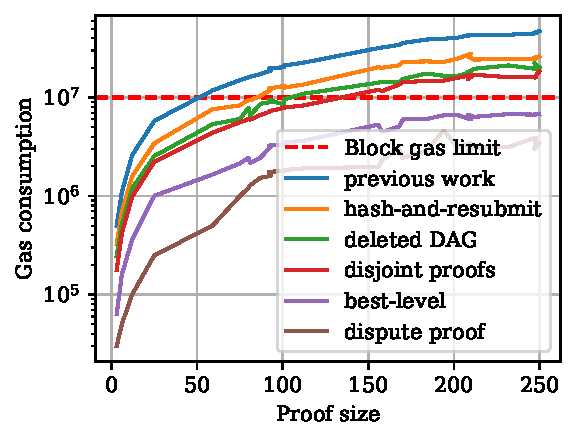
\includegraphics[width=1\columnwidth]{figures/dispute.pdf}
    \end{center}
    \caption{Caption}
    \label{fig:dispute}
\end{figure}
